\chapter{LEVANTAMENTO DE REQUISITOS}

Este capítulo apresenta o levantamento de requisitos realizado para o aplicativo Desconecta, em que o objetivo é auxiliar usuários a reduzirem o tempo de uso do \textit{smartphone} por meio de uma dinâmica em grupo. Para isso, foi realizado um estudo prévio com um grupo restrito de pessoas, no qual foram observados hábitos de uso do celular e aplicado formulário para coleta de informações relevantes ao desenvolvimento do aplicativo. A partir desses dados, foi possível compreender dificuldades enfrentadas pelos usuários e validar a proposta da solução. O formulário, suas respostas completas e os principais registros do grupo de testes estão disponíveis nos Apêndices deste trabalho.

\section{Pesquisa de Informações}

A pesquisa de informações teve como objetivo apoiar o levantamento de requisitos do aplicativo Desconecta, buscando compreender como os participantes utilizam o \textit{smartphone} no dia a dia, quais dificuldades enfrentam para reduzir o tempo de uso e como reagem a uma dinâmica coletiva de acompanhamento. Para isso, foi formado um grupo restrito de seis participantes, que participaram tanto da coleta inicial de dados quanto da experiência prática proposta.

Inicialmente, foi aplicado um formulário online com perguntas voltadas aos hábitos de uso do celular, percepção sobre o tempo de tela, impactos no cotidiano e tentativas anteriores de redução. Esse formulário foi respondido apenas pelos integrantes do grupo, servindo como base para entender o perfil dos participantes e orientar a definição das funcionalidades do aplicativo.

Em seguida, foi realizada uma experiência prática por meio de um grupo no \textit{WhatsApp}, criado para simular a proposta central do aplicativo. Durante aproximadamente uma semana, os participantes compartilharam diariamente seus tempos de uso do celular, além de comentários espontâneos sobre metas, dificuldades e estratégias adotadas para reduzir o tempo de tela. Essa dinâmica permitiu observar, na prática, como a exposição do uso, o acompanhamento diário e a interação em grupo influenciam o comportamento dos usuários.

Os resultados dessa pesquisa são apresentados nas subseções a seguir, abordando o perfil dos participantes, os hábitos e impactos do uso do \textit{smartphone}, as tentativas de redução relatadas e, por fim, as observações obtidas a partir da experiência do grupo de testes.

\subsection{Perfil dos participantes e hábitos de uso}

O estudo contou com a participação de seis usuários adultos, com rotinas distintas envolvendo trabalho, estudo e atividades pessoais. A análise do formulário indicou que 83\% dos participantes consideram que utilizam o celular mais do que gostariam, conforme ilustrado na Figura~\ref{fig:uso_excessivo}. Esse dado aponta uma percepção inicial de uso excessivo entre os integrantes do grupo.

\begin{figure}[htbp]
    \centering
    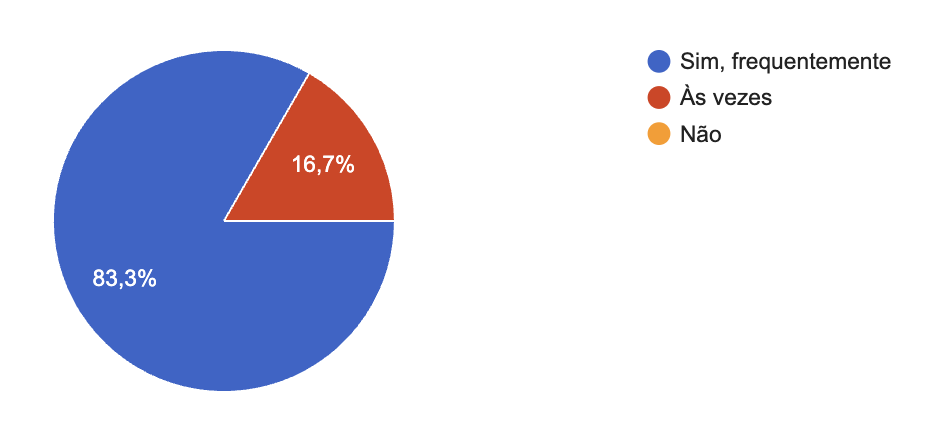
\includegraphics[width=0.6\linewidth]{figuras/uso_excessivo.png}
    \caption{Percepção dos participantes sobre o uso excessivo do celular}
    \label{fig:uso_excessivo}
\end{figure}

Em relação aos hábitos de uso, 83\% afirmaram usar o celular principalmente por hábito ou tédio, e não necessariamente por uma necessidade específica, como mostra a Figura~\ref{fig:uso_sem_motivo}. Os aplicativos mais citados como responsáveis pelo maior tempo de uso foram redes sociais e plataformas de vídeos curtos, como \textit{Instagram}, \textit{TikTok} e conteúdos de \textit{reels} e \textit{memes}.

\begin{figure}[htbp]
    \centering
    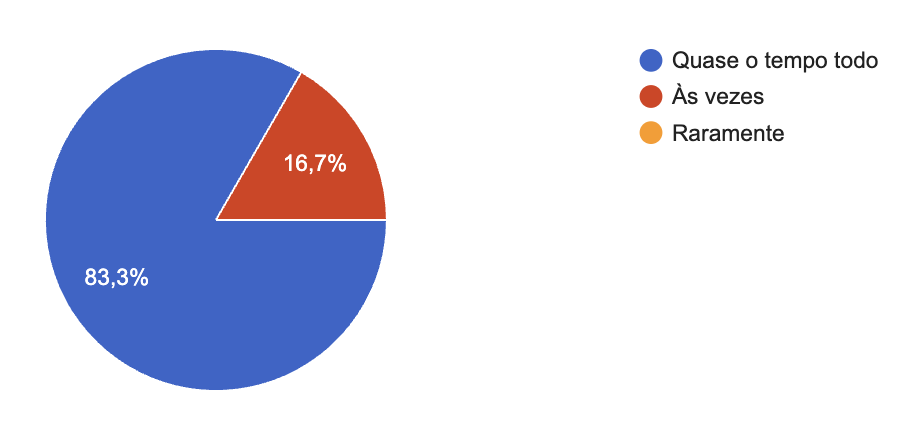
\includegraphics[width=0.6\linewidth]{figuras/uso_sem_motivo.png}
    \caption{Frequência de uso do celular sem motivo específico}
    \label{fig:uso_sem_motivo}
\end{figure}

Esses dados quantitativos são reforçados por comentários feitos no grupo de testes, nos quais participantes relataram que o consumo de vídeos curtos ocorre de forma automática, muitas vezes sem perceber a passagem do tempo, como no relato “fico ali vidrado e quando vejo já se passaram horas”.

\subsection{Impactos percebidos do uso excessivo}

Os impactos emocionais e comportamentais do uso excessivo também foram investigados. Conforme apresentado na Figura~\ref{fig:ansiedade_longe_celular}, mais da metade dos participantes relatou já ter sentido ansiedade ou desconforto ao ficar longe do celular, o que indica possível dependência comportamental.

\begin{figure}[htbp]
    \centering
    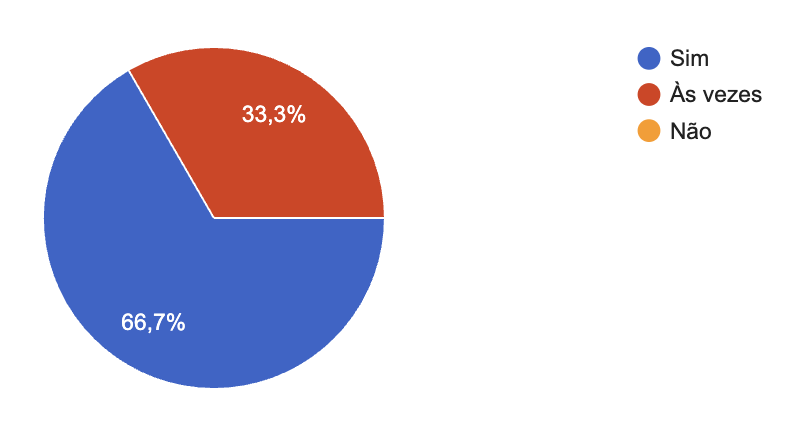
\includegraphics[width=0.5\linewidth]{figuras/ansiedade_longe_celular.png}
    \caption{Participante já sentiu ansiedade ou desconforto ao ficar longe do celular}
    \label{fig:ansiedade_longe_celular}
\end{figure}

Além disso, a Figura~\ref{fig:situacoes_mais_frequentes} apresenta as situações em que o uso excessivo ocorre com maior frequência, em que é possível notar maior uso em momentos de tédio, antes de dormir e em intervalos ao longo do dia.

\begin{figure}[htbp]
    \centering
    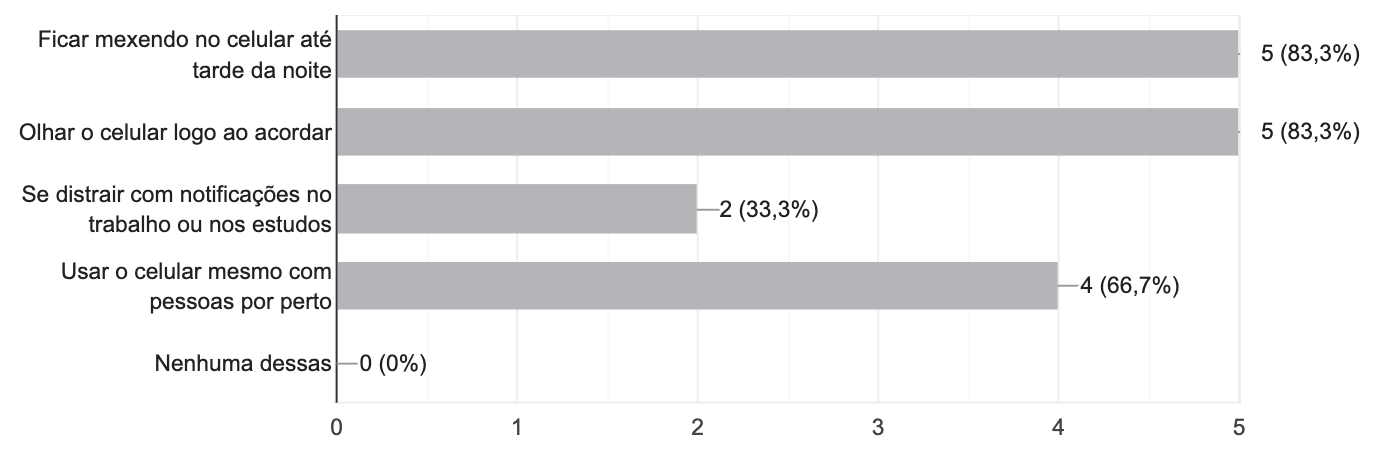
\includegraphics[width=0.8\linewidth]{figuras/situacoes_mais_frequentes.png}
    \caption{Situações nas quais o uso é mais frequente}
    \label{fig:situacoes_mais_frequentes}
\end{figure}

Esses impactos foram confirmados na prática durante a primeira etapa de avaliação do grupo. Os participantes relataram que a exposição diária do tempo de uso passou a gerar um senso de responsabilidade em relação ao envio dos dados no grupo, influenciando diretamente a mudança de comportamento coletiva. Saber que outras pessoas estavam acompanhando os resultados passou a influenciar decisões mais conscientes sobre o uso do celular, funcionando como incentivo para reduzir o tempo de tela.

\begin{figure}[htbp]
    \centering
    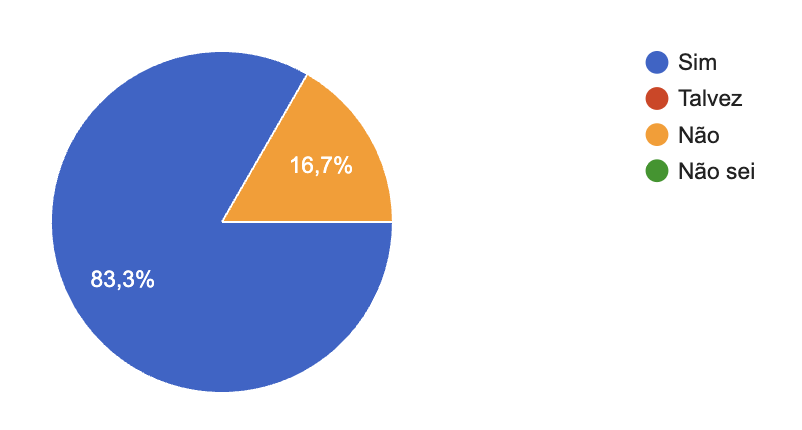
\includegraphics[width=0.5\linewidth]{figuras/visibilidade_social.png}
    \caption{Influência da visibilidade do tempo de uso na redução do uso do celular}
    \label{fig:visibilidade_social}
\end{figure}

Conforme ilustrado na Figura~\ref{fig:visibilidade_social}, 83,3\% dos participantes afirmaram que utilizariam menos o celular caso outras pessoas pudessem visualizar seu tempo de uso, confirmando essa influência. Esse resultado está alinhado com os depoimentos observados ao longo dessa primeira etapa de avaliação.

Relatos como “as cinco horas de ontem no celular me assustaram, tava perdendo muito tempo” e “quando eu ocupo a cabeça com outras coisas mexo menos no celular” ilustram esse efeito. Também houve comentários indicando tentativa consciente de mudança, como “fiz algumas mudanças hoje e mais tarde mostro o resultado” e “desativei várias notificações no meu celular”, demonstrando que o compartilhamento coletivo contribuiu para maior reflexão sobre os próprios hábitos.

Também foi possível observar variações claras entre dias mais produtivos e dias ociosos. Participantes relataram que, em dias com trabalho, estudo ou atividades externas, o tempo de uso foi menor, enquanto dias sem rotina definida resultaram em aumento significativo do tempo de tela.

\subsection{Tentativas de redução do tempo de uso}

Conforme ilustrado na Figura~\ref{fig:oq_mais_motiva_usar_menos}, a principal motivação apontada pelos participantes para reduzir o tempo de uso está relacionada a aumentar foco e produtividade. O resultado sugere que a preocupação não está apenas na quantidade de horas gastas no celular, mas principalmente nos impactos percebidos na rotina, no desempenho das atividades diárias e no bem-estar geral.

\begin{figure}[htbp]
    \centering
    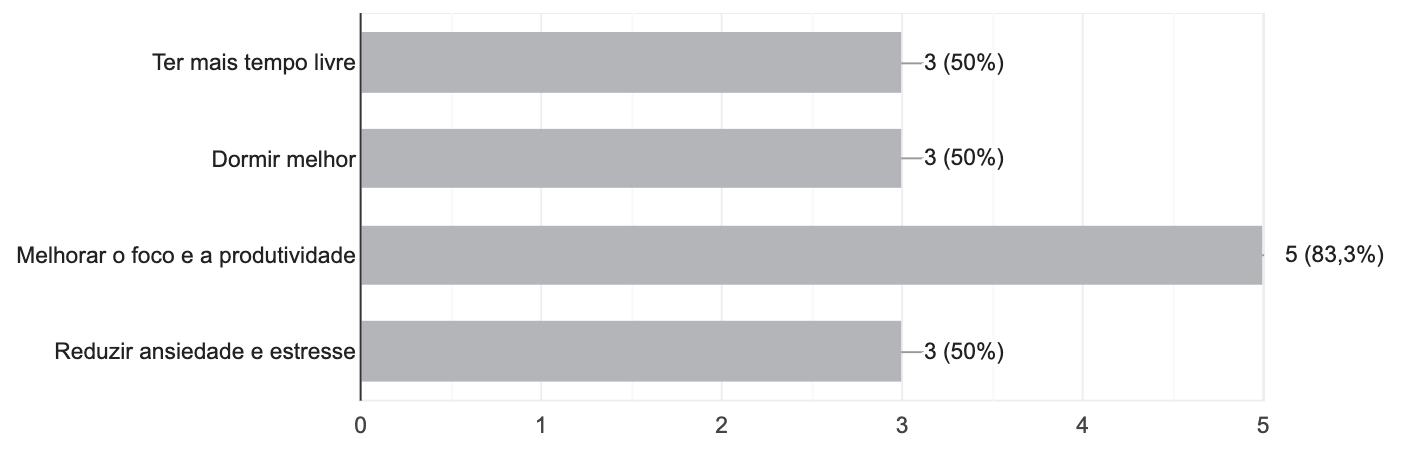
\includegraphics[width=0.8\linewidth]{figuras/oq_mais_motiva_usar_menos.png}
    \caption{O que mais motiva a usar menos o celular}
    \label{fig:oq_mais_motiva_usar_menos}
\end{figure}

Além disso, como mostra a Figura~\ref{fig:ja_tentou_reduzir_sozinho}, 83\% dos participantes já tentaram reduzir o tempo de uso por conta própria, porém relataram dificuldade em manter essas mudanças por longos períodos.

\begin{figure}[htbp]
    \centering
    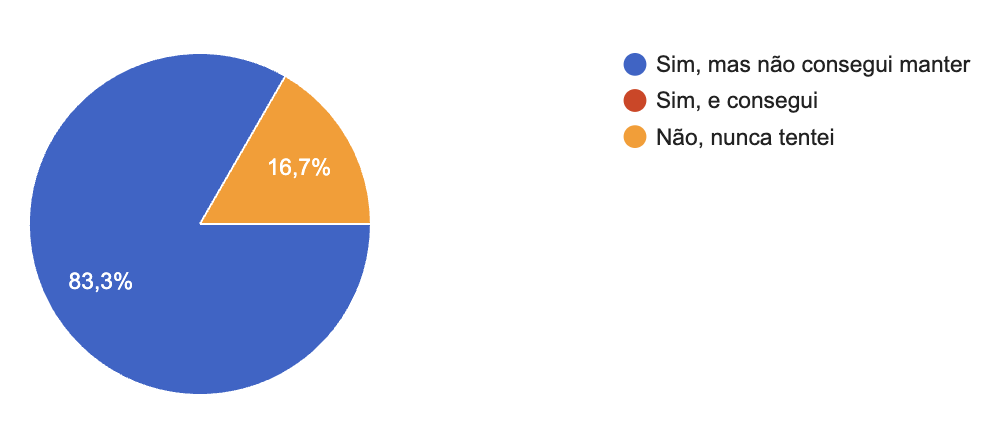
\includegraphics[width=0.7\linewidth]{figuras/ja_tentou_reduzir_sozinho.png}
    \caption{Tentativa de redução por conta própria}
    \label{fig:ja_tentou_reduzir_sozinho}
\end{figure}

Durante a primeira etapa de avaliação em grupo, essas tentativas tornaram-se mais concretas. Um dos participantes, por exemplo, estabeleceu mudanças simples, como evitar o uso do celular ao acordar, limitar o uso de redes sociais a três horas diárias, evitar o uso do celular na academia e não usar o dispositivo na realização de outras tarefas, como no momento das refeições e tarefas domésticas.

\begin{figure}[htbp]
    \centering
    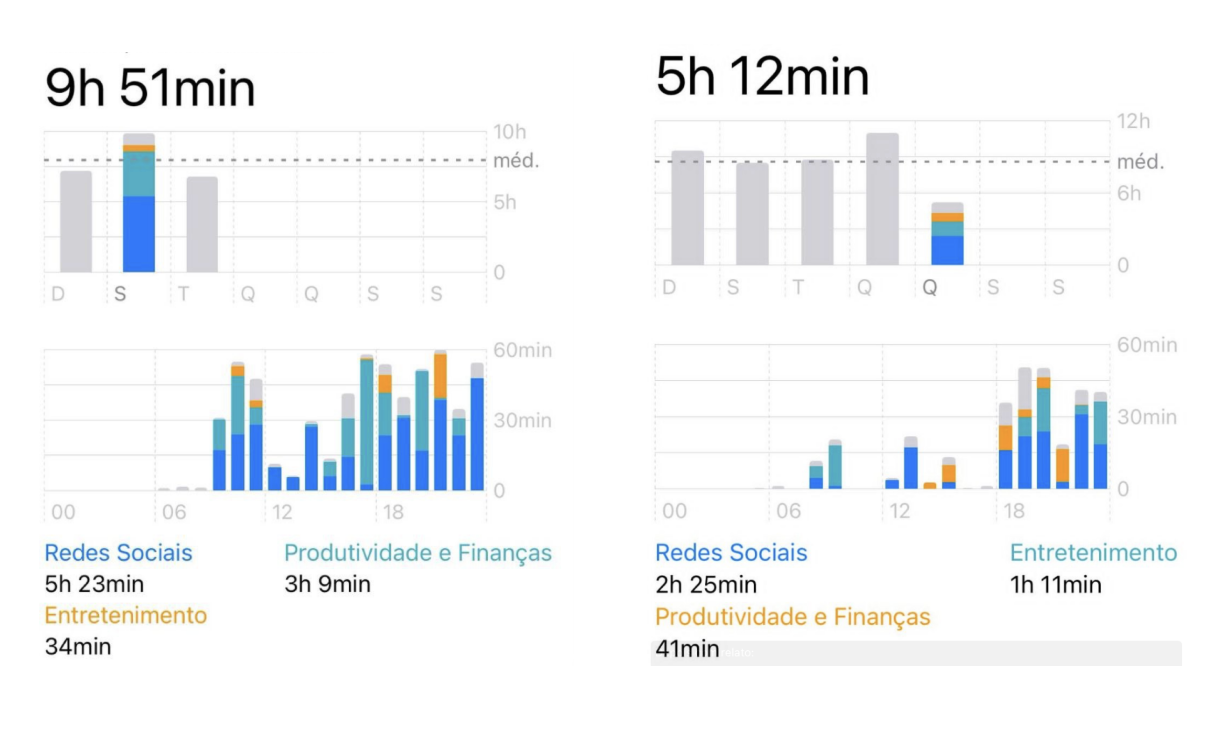
\includegraphics[width=0.7\linewidth]{figuras/uso_antes_depois_mudanca.png}
    \caption{Tempo de uso de uma pessoa participante em específico antes (esquerda) e depois (direita) da aplicação das mudanças}
    \label{fig:uso_antes_depois_mudanca}
\end{figure}

Após alguns dias aplicando essas estratégias, foi possível observar, no caso dessa pessoa participante em específico, uma redução no tempo total de uso, conforme ilustrado na Figura~\ref{fig:uso_antes_depois_mudanca}. Inclusive, o relato “são mudanças simples, mas fizeram diferença para mim”, evidencia que pequenas intervenções comportamentais, quando acompanhadas coletivamente, podem gerar bons resultados.

\subsection{Dinâmica e observações do grupo de testes}

O formulário indicou uma forte aceitação da proposta de acompanhamento em grupo. Todos os participantes afirmaram acreditar que uma dinâmica coletiva pode auxiliar na redução do tempo de uso do celular. Além disso, como ilustrado na Figura~\ref{fig:motivacao_comparacao}, 66\% afirmaram que se sentem motivados ao ver o tempo de tela de outras pessoas, enquanto os demais indicaram sentir ao menos algum nível de influência positiva.

\begin{figure}[htbp]
    \centering
    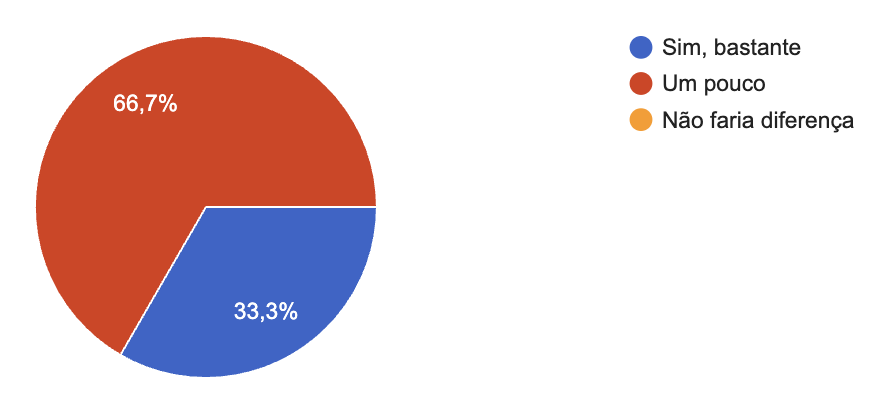
\includegraphics[width=0.6\linewidth]{figuras/motivacao_comparacao.png}
    \caption{Motivação ao ver outras pessoas compartilhando próprio tempo de tela}
    \label{fig:motivacao_comparacao}
\end{figure}

Quando questionados sobre quais elementos tornariam a experiência coletiva mais eficaz, os participantes destacaram principalmente incentivo e lembretes, metas diárias e a possibilidade de acompanhar o progresso dos demais integrantes do grupo, conforme apresentado na Figura~\ref{fig:elementos_grupo}. Esses resultados reforçam que o engajamento coletivo não depende apenas da existência do grupo, mas também da presença de mecanismos estruturados de acompanhamento e estímulo contínuo.

\begin{figure}[htbp]
    \centering
    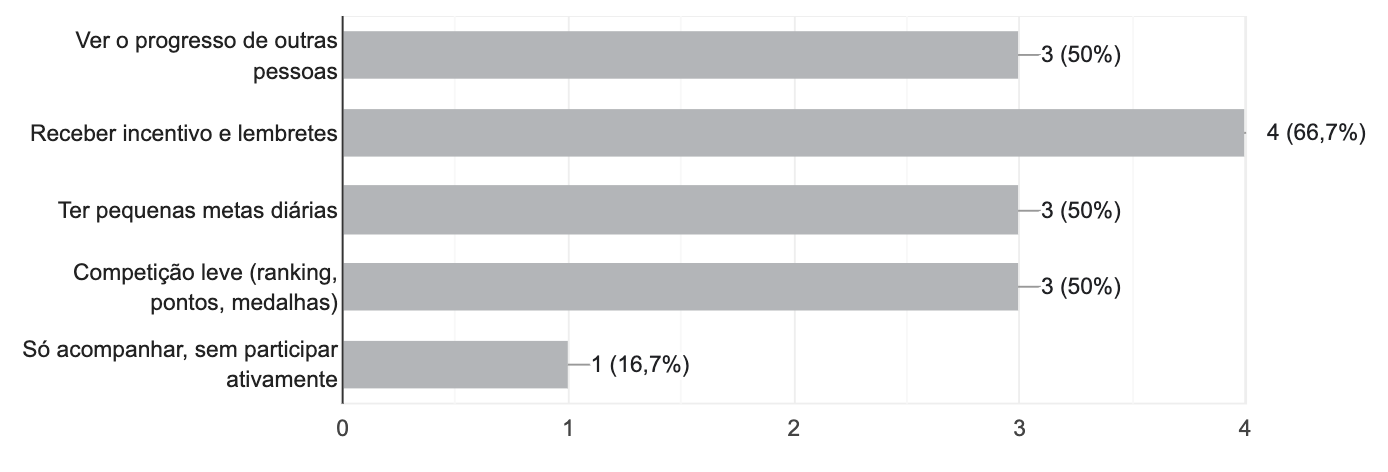
\includegraphics[width=0.9\linewidth]{figuras/elementos_grupo.png}
    \caption{O que mais ajuda em um grupo focado em usar menos o celular}
    \label{fig:elementos_grupo}
\end{figure}

\section{Requisitos da Solução Proposta}

Com base na proposta de reduzir o uso de telas e promover hábitos digitais mais saudáveis, foram definidos os seguintes \textbf{requisitos funcionais} do aplicativo Desconecta:

\begin{enumerate}
    \item Ser uma plataforma acessível e fácil de usar, com foco na simplicidade.
    \item Permitir o acompanhamento do tempo de uso diário do celular.
    \item Mostrar comparações de uso, como tempo gasto em relação ao dia ou semana anterior.
    \item Exibir o tempo gasto em cada aplicativo, sempre que possível.
    \item Caso o sistema do celular não permita essa medição automaticamente, oferecer uma forma simples para o usuário registrar seu tempo manualmente.
    \item Enviar alertas quando o tempo de uso ultrapassar limites definidos pelo próprio usuário ou estiver chegando perto do limite.
    \item Apresentar níveis de “saúde digital”, ajudando a identificar padrões de uso equilibrado ou excessivo.
    \item Permitir que o usuário crie e personalize seu perfil (nome, foto e breve descrição).
    \item Possibilitar a definição de metas pessoais, como limite de tempo diário ou horários sem celular.
    \item Permitir a criação de grupos de amigos para incentivar desafios coletivos.
    \item Permitir que cada grupo escolha suas próprias regras, como:
    \begin{itemize}
        \item Competição por menor tempo de tela;
        \item Sistema de pontuação;
        \item Metas personalizadas do grupo.
    \end{itemize}
    \item Exibir rankings que mostram a comparação entre os membros do grupo.
    \item Oferecer rankings gerais, permitindo que o usuário saiba onde ele se encontra em relação à média de todos os usuários da plataforma.
    \item Disponibilizar desafios coletivos maiores, como ações por bairro, cidades ou regiões, incentivando práticas de desconexão digital.
\end{enumerate}